\chapter{Lagrangian Examples and Hamiltonian Motion}

This lecture begins in a practical register. Leonard Susskind does not first advertise elegance; he wants to show that the Lagrangian method turns awkward constrained systems into a disciplined procedure. We choose coordinates, write \(L=T-V\), and then let the equations of motion and conservation laws emerge. These notes follow that movement closely, from two concrete examples to the Hamiltonian formulation and finally to the harmonic oscillator in phase space. The selected board captures kept in this chapter were curated for this edition by LazyingArt LLC and Video2Book.

\section{Why Lagrangians Are Powerful}

The first claim is deliberately modest, but it is the right claim. To solve a mechanics problem, for the purposes of this lecture, does not necessarily mean to integrate the motion in closed form. It means to write down the equations of motion. Once those are known, one can always turn them over to numerical methods. What is difficult, and what the Lagrangian formalism simplifies, is the act of setting the problem up correctly.

That is why Susskind likes these examples. By Newton's laws one could certainly solve them, but one would have to follow the internal forces and the constraints in detail. By the Lagrangian method the calculation becomes almost algorithmic. Once the rules are known, much of the work is mechanical.

There is, however, one non-mechanical step at the beginning: we must choose coordinates. And the lecture immediately reminds us what coordinates are for. They do not describe the whole motion. They label an instantaneous configuration.

\subsection{Question \& Answer}

\paragraph{Question.} What does it mean, here, to solve a mechanics problem?

\paragraph{Answer.} It means to find the equations of motion. If those equations have been written down correctly, then the mechanical problem is already under control, even if the later integration is numerical rather than explicit.

\section{Sliding Wedge: Coordinates, \(T-V\), and Conserved Momentum}

The first example is a wedge of mass \(M\) sliding without friction along a horizontal surface, together with a point particle of mass \(m\) constrained to move along the face of the wedge. The whole point of the example is to make the workflow visible.

We first choose coordinates. The lecture emphasizes that this choice is not unique. One needs only enough coordinates to label the instantaneous configuration, and they should not be redundant. Susskind chooses
\begin{equation}
\begin{aligned}
X&=\text{horizontal position of the wedge corner},\\
x&=\text{particle's horizontal position relative to that corner}.
\end{aligned}
\end{equation}
For a wedge of fixed slope one has, in general,
\begin{equation}
\frac{y}{x}=\tan\beta,
\end{equation}
where \(\beta\) is the wedge angle. To keep the example clean, the lecture specializes to \(\beta=45^\circ\), so that
\begin{equation}
y=x,\qquad \dot y=\dot x.
\end{equation}

Now we write \(T-V\). The wedge moves only horizontally, so its kinetic energy is
\begin{equation}
T_{\text{wedge}}=\frac12 M\dot X^2.
\end{equation}
The particle has two velocity components. Its horizontal component is \(\dot X+\dot x\), because the wedge itself is moving, and in the \(45^\circ\) example its vertical component is \(\dot x\). Therefore
\begin{equation}
T_{\text{particle}}=\frac m2\Big[(\dot X+\dot x)^2+\dot x^2\Big].
\end{equation}
The potential energy comes only from the particle, and in this special geometry its height is just \(x\):
\begin{equation}
V=mgx.
\end{equation}
So the Lagrangian is
\begin{equation}
L=\frac12 M\dot X^2+\frac m2\Big[(\dot X+\dot x)^2+\dot x^2\Big]-mgx.
\end{equation}

At this point the lecture does not push hard on solving both equations of motion. Instead it turns to canonical momentum, because this is where the formalism begins to show its real power. By definition,
\begin{align}
p_X&=\frac{\partial L}{\partial \dot X}
   =M\dot X+m(\dot X+\dot x),\\
p_x&=\frac{\partial L}{\partial \dot x}
   =m(\dot X+\dot x)+m\dot x.
\end{align}
This is where one must resist ordinary intuition. Canonical momentum is not simply whichever \(mv\) one might first guess. It is defined by
\begin{equation}
p_i=\frac{\partial L}{\partial \dot q_i}.
\end{equation}
In constrained systems that distinction matters.

Now the symmetry is easy to see. A horizontal translation of the whole system acts by
\begin{equation}
\delta X=\epsilon,\qquad \delta x=0.
\end{equation}
More generally, if a symmetry acts as
\begin{equation}
\delta q_i=\epsilon f_i,
\end{equation}
then the corresponding conserved quantity is
\begin{equation}
Q=\sum_i p_i f_i.
\end{equation}
Here \(f_X=1\) and \(f_x=0\), so the Noether quantity is simply
\begin{equation}
Q=p_X.
\end{equation}
Equivalently, \(X\) is a cyclic coordinate, so
\begin{equation}
\dot p_X=\frac{\partial L}{\partial X}=0.
\end{equation}
This is the conservation law the lecture wants us to notice. We never had to solve for the constraint forces between wedge and particle.

For completeness, the other Euler--Lagrange equation is
\begin{equation}
\dot p_x=\frac{\partial L}{\partial x}=-mg.
\end{equation}
The lecture hesitates over the sign and then fixes it. The safe statement is the canonical one: since \(L=T-V\), the explicit \(x\)-dependence comes from \(-V\), so \(\partial L/\partial x=-\,\partial V/\partial x\).

There is no analogous vertical conservation law. The wedge is not free to translate vertically, and motion in that direction changes the potential energy. The horizontal symmetry survives; the vertical one does not.

\section{Double Pendulum: Choosing the Right Angles}

The second example is the double pendulum, and here the lecture slows down at exactly the right place. The issue is not yet algebra. The issue is how to choose coordinates so that the structure of the problem is visible.

We take both rods to have unit length and both bobs to have unit mass. The first angle is naturally called \(\theta\). For the second rod there are two natural choices. One could measure its angle from the vertical and call it, say, \(\phi\). Or one could measure it relative to the first rod and call that relative angle \(\alpha\).

Susskind chooses \(\alpha\), the relative angle, and he tells us why before calculating anything. Forget gravity for a moment. Then the whole double pendulum has an obvious rotational symmetry. If we rotate the entire apparatus rigidly, the relative angle between the rods does not change. In that coordinate system the symmetry acts simply:
\begin{equation}
\theta\to \theta+\epsilon,\qquad \alpha\to \alpha.
\end{equation}
That is the advantage. The symmetry shifts one coordinate and leaves the other fixed.

This is one of the places where the lecture is careful about the role of cleverness. If our only goal were to write down equations of motion and put them on a computer, almost any reasonable coordinates would do. But if we want the symmetry to announce itself immediately, then the coordinate choice matters.

\subsection{Question \& Answer}

\paragraph{Question.} Why is the second angle measured relative to the first rod rather than relative to the vertical?

\paragraph{Answer.} Because in the no-gravity problem the rotational symmetry then acts only on \(\theta\) and leaves \(\alpha\) fixed. That makes \(\theta\) the cyclic coordinate. With the vertical-angle choice both coordinates would transform under the symmetry, and the conserved quantity would be less transparent even though the physics would be the same.

\section{Double Pendulum: Kinematics, Cyclic Coordinates, and Gravity}

Having chosen \((\theta,\alpha)\), Susskind computes the kinetic energy by a useful detour through Cartesian coordinates. The first bob has coordinates
\begin{equation}
x=\sin\theta,\qquad y=\cos\theta,
\end{equation}
with \(y\) measured downward. Differentiating,
\begin{equation}
\dot x=\dot\theta\cos\theta,\qquad \dot y=-\dot\theta\sin\theta.
\end{equation}
So the first bob contributes
\begin{equation}
\dot x^{\,2}+\dot y^{\,2}=\dot\theta^{\,2}
\end{equation}
to the kinetic-energy algebra.

For the second bob we introduce
\begin{equation}
x'=\sin\theta+\sin(\theta+\alpha),\qquad
y'=\cos\theta+\cos(\theta+\alpha).
\end{equation}
A representative velocity component is
\begin{equation}
\dot x'=\dot\theta\cos\theta+(\dot\theta+\dot\alpha)\cos(\theta+\alpha),
\end{equation}
and similarly for \(\dot y'\). One then adds \(x'^2\)- and \(y'^2\)-type terms, simplifies with trigonometric identities, and rewrites the result in angular variables.

This is where the lecture becomes intentionally informal. The algebra is straightforward but messy, and the sign convention in the mixed \(\dot\theta\)--\(\dot\alpha\) terms is explicitly challenged from the audience. A late board state preserves one lecture-local line,
\begin{equation}
T-V=\dot\theta^{\,2}+\frac{(\dot\theta-\dot\alpha)^2}{2}
+\dot\theta(\dot\theta-\dot\alpha)\cos\alpha,
\end{equation}
but this should be read cautiously. The lecture itself admits that one of the \(\dot\theta\pm\dot\alpha\) signs may be wrong depending on how the positive direction of \(\alpha\) was chosen. The important point is not that exact local sign, but the symmetry structure.

\begin{figure}[htbp]
\centering

\includegraphics[width=0.82\textwidth]{lecture_06_figure_02.png}
\caption{Double-pendulum board work: a lecture-local \(T-V\) line above and the \(\theta\)-equation below. The board writes \(P_\theta\); in the notes we use the standard lowercase \(p_\theta\).}
\end{figure}

The clean statement is the Euler--Lagrange one:
\begin{equation}
\dot p_\theta=\frac{\partial L}{\partial \theta}.
\end{equation}
Now comes the payoff of the coordinate choice. In the absence of gravity, \(\theta\) does not appear explicitly in the Lagrangian. Therefore
\begin{equation}
\frac{\partial L}{\partial \theta}=0,
\end{equation}
and hence
\begin{equation}
\dot p_\theta=0.
\end{equation}
The conserved quantity is the total angular momentum of the two-bob system.

This is also where the lecture answers a natural misconception. The conservation of \(p_\theta\) does not mean that \(\dot\theta\) and \(\dot\alpha\) are separately constant. The two bobs exchange angular momentum through the rods, exactly as two masses on a spring exchange ordinary momentum. What is conserved is one particular combination, not the individual angular velocities.

With gravity restored, the rotational symmetry is broken. The potential energy is built from the heights of both bobs, and in this coordinate system it takes the schematic form
\begin{equation}
V_{\text{grav}}\propto \cos\theta+\cos(\theta+\alpha),
\end{equation}
up to overall sign and normalization conventions that depend on whether one measures \(y\) upward or downward and whether one is writing \(V\) or \(L=T-V\). The lecture does not polish this point into a canonical formula; it only wants the physical lesson: once gravity is present, \(\theta\) is no longer cyclic, so the free-rotation conservation law is lost.

At this stage Susskind also remarks on a separate audience question: chaos is not something one usually sees at a glance from the equations themselves. One may change parameters and pass from non-chaotic to chaotic behavior, but there is no simple visual criterion sitting in the raw formulas.

\subsection{Question \& Answer}

\paragraph{Question.} Is \(\dot p_i=0\) in every conservative system?

\paragraph{Answer.} No. In general the Euler--Lagrange equation says
\begin{equation}
\dot p_i=\frac{\partial L}{\partial q_i}.
\end{equation}
Only when the coordinate \(q_i\) is cyclic, so that \(L\) has no explicit dependence on it, does the right-hand side vanish. If \(L=T-V\) and \(T\) has no explicit \(q_i\)-dependence, then one gets the more familiar form
\begin{equation}
\dot p_i=-\frac{\partial V}{\partial q_i}.
\end{equation}
So \(\dot p_i=0\) is a special case, not a universal one.

\section{Hamiltonian Mechanics as a New Formulation}

Only after these two examples does the lecture turn to the Hamiltonian. The Hamiltonian is first introduced in its familiar role: it is the conserved energy. But Susskind immediately broadens the point. The Hamiltonian is also the basis of a third formulation of mechanics, alongside Newton's equations and the Euler--Lagrange form of the principle of least action.

The change of viewpoint is decisive. In the Lagrangian language we think in terms of \(q_i\) and \(\dot q_i\). In the Hamiltonian language we think in terms of \(q_i\) and \(p_i\). The momenta are no longer odd derivatives that sit off to the side. They stand on almost the same footing as the coordinates themselves.

The defining formula is
\begin{equation}
H=\sum_i \dot q_i p_i-L.
\end{equation}
For a good mechanical system one should be able to solve the momentum-velocity relations and write the \(\dot q_i\) as functions of \(q_i\) and \(p_i\). Then the Hamiltonian is properly regarded as a function \(H(q,p)\).

At this point Susskind reaches back to the first lecture and recalls a geometric moral. A reversible law of motion cannot have many states collapsing into one future state, nor one state branching into many futures. In the language that Hamiltonian mechanics will make precise, the flow in phase space should have neither convergence into sinks nor divergence out of sources. He does not prove that yet, but he wants us to keep the picture in mind.

Before deriving the general equations, he does what he usually does when a formalism threatens to become abstract: he turns immediately to an example.

\section{A First Look at the Oscillator Hamiltonian and Phase Space}

The example is the harmonic oscillator. Susskind chooses to write its Lagrangian in the rescaled form
\begin{equation}
L=\frac{1}{2\omega}\dot q^{\,2}-\frac{\omega}{2}q^2,
\end{equation}
where \(\omega\) is the oscillator frequency. This is not the most familiar form, but it is chosen for a reason.

We may begin from the ordinary oscillator,
\begin{equation}
L=\frac12 m\dot x^2-\frac12 kx^2,\qquad \omega=\sqrt{\frac{k}{m}}.
\end{equation}
Now define a new coordinate \(q\) so that the potential term becomes symmetric with the eventual momentum term:
\begin{equation}
\frac{\omega}{2}q^2=\frac{k}{2}x^2.
\end{equation}
Hence
\begin{equation}
q^2=\sqrt{km}\,x^2.
\end{equation}
One consistent choice is \(q=(km)^{1/4}x\), and then
\begin{equation}
\dot q^{\,2}=\sqrt{km}\,\dot x^{\,2}.
\end{equation}
With that substitution the kinetic term also takes the desired form, and the oscillator Lagrangian becomes
\begin{equation}
L=\frac{1}{2\omega}\dot q^{\,2}-\frac{\omega}{2}q^2.
\end{equation}

The price is that \(q\) is no longer a literal length. This is an explicit theme in the lecture's later discussion of units. The reward is that the Hamiltonian becomes symmetric in \(q\) and \(p\).

The momentum conjugate to the rescaled coordinate is
\begin{equation}
p=\frac{\partial L}{\partial \dot q}=\frac{\dot q}{\omega},
\end{equation}
so
\begin{equation}
\dot q=\omega p.
\end{equation}
Now compute the Hamiltonian:
\begin{align}
H(q,p)
&=\dot q\,p-L \\
&=(\omega p)p-\left[\frac{1}{2\omega}(\omega^2p^2)-\frac{\omega}{2}q^2\right] \\
&=\frac{\omega}{2}(p^2+q^2).
\end{align}
That is the crucial simplification. The rescaling was chosen precisely so that the same \(\omega/2\) multiplies both \(p^2\) and \(q^2\).

Constant energy therefore means
\begin{equation}
p^2+q^2=\frac{2H}{\omega},
\end{equation}
so the constant-energy curves in the \((q,p)\) plane are circles. That is the first real geometric payoff of the Hamiltonian viewpoint.

\begin{figure}[htbp]
\centering

\includegraphics[width=0.74\textwidth]{lecture_06_figure_04.png}
\caption{The late phase-space board sketch: nested closed trajectories, a marked point on an outer orbit, and a cloud of sample points filling part of the annular region.}
\end{figure}

\begin{figure}[htbp]
\centering
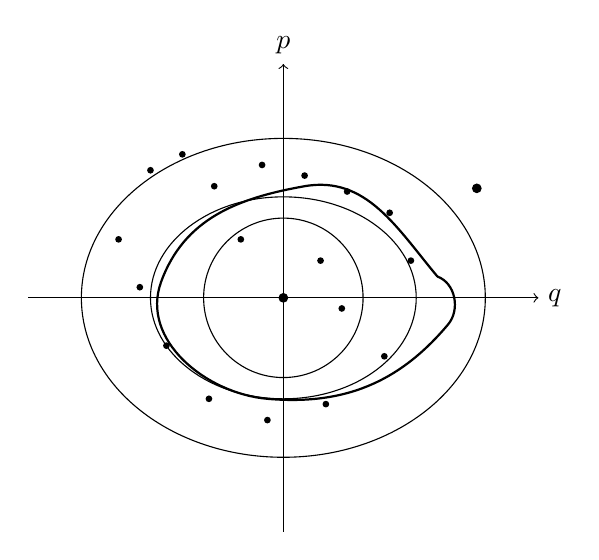
\begin{tikzpicture}[scale=1.35]
\draw[->] (-2.4,0) -- (2.4,0) node[right] {$q$};
\draw[->] (0,-2.2) -- (0,2.2) node[above] {$p$};
\draw (0,0) circle (0.75);
\draw (0,0) ellipse (1.25 and 0.95);
\draw (0,0) ellipse (1.9 and 1.5);
\draw[thick] (1.45,0.2)
  to[out=130,in=10] (0.2,1.05)
  to[out=190,in=70] (-1.15,0.15)
  to[out=-110,in=175] (-0.15,-0.95)
  to[out=-5,in=-130] (1.55,-0.25)
  to[out=50,in=-20] (1.45,0.2);
\fill (0,0) circle (1.3pt);
\fill (1.82,1.03) circle (1.3pt);
\fill (-1.25,1.20) circle (0.9pt);
\fill (-1.55,0.55) circle (0.9pt);
\fill (-0.95,1.35) circle (0.9pt);
\fill (-0.65,1.05) circle (0.9pt);
\fill (-0.20,1.25) circle (0.9pt);
\fill (0.20,1.15) circle (0.9pt);
\fill (0.60,1.00) circle (0.9pt);
\fill (1.00,0.80) circle (0.9pt);
\fill (1.20,0.35) circle (0.9pt);
\fill (0.95,-0.55) circle (0.9pt);
\fill (0.40,-1.00) circle (0.9pt);
\fill (-0.15,-1.15) circle (0.9pt);
\fill (-0.70,-0.95) circle (0.9pt);
\fill (-1.10,-0.45) circle (0.9pt);
\fill (-1.35,0.10) circle (0.9pt);
\fill (-0.40,0.55) circle (0.9pt);
\fill (0.35,0.35) circle (0.9pt);
\fill (0.55,-0.10) circle (0.9pt);
\end{tikzpicture}
\caption{A cleaned phase-space redraw based on the board sketch. The lecture's point is not the exact shape of the hand-drawn curves but the existence of closed energy shells and a whole cloud of initial conditions transported by the same flow.}
\end{figure}

If we had stayed with the original variables \((x,p_x)\), we would instead have
\begin{equation}
H(x,p_x)=\frac{p_x^2}{2m}+\frac{k}{2}x^2,
\end{equation}
so the constant-energy curves would be ellipses. The change of variables is therefore not cosmetic. It is chosen to make the symmetry between coordinate and momentum visible. This is also where the units discussion comes from: the rescaled \(q\) is an abstract coordinate, and the conjugate \(p\) is not the same object as the ordinary mechanical momentum \(p_x\).

Already, before any general derivation, we see the Hamiltonian way of thinking. Motion is not merely back and forth in \(q\). It is motion in the \((q,p)\) plane, trapped on a circle by energy conservation.

\section{Deriving Hamilton's Equations and Returning to the Oscillator}

After that geometric preview, Susskind returns to the formal question: what are the equations of motion in the Hamiltonian formulation?

He begins with the standard trick from multivariable calculus. If \(F\) is a function of the variables \(q_i\) and \(p_i\), then a small change in those variables produces
\begin{equation}
\delta F=\sum_i\left(\frac{\partial F}{\partial q_i}\delta q_i+\frac{\partial F}{\partial p_i}\delta p_i\right).
\end{equation}
Conversely, if we can write \(\delta F\) in the form \(A_i\delta q_i+B_i\delta p_i\), then the coefficients must be the partial derivatives.

Now apply that idea directly to the Hamiltonian
\begin{equation}
H=\sum_i \dot q_i p_i-L.
\end{equation}
We vary everything that can vary:
\begin{align}
\delta H
&=\sum_i\big(\dot q_i\,\delta p_i+p_i\,\delta\dot q_i\big)
-\sum_i\left(\frac{\partial L}{\partial \dot q_i}\delta\dot q_i+\frac{\partial L}{\partial q_i}\delta q_i\right).
\end{align}
But by definition,
\begin{equation}
\frac{\partial L}{\partial \dot q_i}=p_i,
\end{equation}
so the \(p_i\,\delta\dot q_i\) terms cancel. Then Euler--Lagrange gives
\begin{equation}
\frac{\partial L}{\partial q_i}=\dot p_i.
\end{equation}
Therefore
\begin{equation}
\delta H=\sum_i \dot q_i\,\delta p_i-\dot p_i\,\delta q_i.
\end{equation}
Comparing with the general variation formula, we read off Hamilton's equations:
\begin{equation}
\frac{\partial H}{\partial p_i}=\dot q_i,\qquad
\frac{\partial H}{\partial q_i}=-\dot p_i.
\end{equation}

\begin{figure}[htbp]
\centering

\includegraphics[width=0.72\textwidth]{lecture_06_figure_03.png}
\caption{The board layout for the Hamiltonian derivation: the defining relation above, the variation line in the middle, and the boxed canonical equations below.}
\end{figure}

This is the formal center of the lecture. The Hamiltonian equations are first order in time. For \(n\) degrees of freedom there are \(2n\) of them. By contrast, the Euler--Lagrange equations are second order, and there are only \(n\). The two descriptions carry the same information, but they distribute it differently.

Now we return to the oscillator. With
\begin{equation}
H=\frac{\omega}{2}(p^2+q^2),
\end{equation}
Hamilton's equations immediately give
\begin{equation}
\dot q=\frac{\partial H}{\partial p}=\omega p,
\end{equation}
and
\begin{equation}
\dot p=-\frac{\partial H}{\partial q}=-\omega q.
\end{equation}
One may almost regard the first as defining \(p\) in terms of the velocity, while the second tells us how that momentum changes.

\subsection{Question \& Answer}

\paragraph{Question.} How can two first-order Hamilton equations be equivalent to one second-order Euler--Lagrange equation?

\paragraph{Answer.} Simply differentiate one and substitute into the other. From
\begin{equation}
\dot q=\omega p
\end{equation}
we get
\begin{equation}
\ddot q=\omega \dot p.
\end{equation}
Using the second Hamilton equation,
\begin{equation}
\dot p=-\omega q,
\end{equation}
we obtain
\begin{equation}
\ddot q=-\omega^2 q.
\end{equation}
That is precisely the standard harmonic-oscillator equation.

The lecture then goes back and writes the same thing in Euler--Lagrange form, without introducing \(p\) at all:
\begin{equation}
\frac{d}{dt}\!\left(\frac{\dot q}{\omega}\right)=-\omega q,
\end{equation}
or
\begin{equation}
\frac{\ddot q}{\omega}=-\omega q.
\end{equation}
Multiply by \(\omega\), and one is back to
\begin{equation}
\ddot q=-\omega^2 q.
\end{equation}
So the Lagrangian description gives one second-order equation for each coordinate, while the Hamiltonian description gives one first-order equation for each coordinate and one for each momentum.

\begin{figure}[htbp]
\centering

\includegraphics[width=0.92\textwidth]{lecture_06_figure_05.png}
\caption{The board state that juxtaposes geometry and equations: phase-space motion on the left, the rescaled oscillator Lagrangian and second-order form on the right.}
\end{figure}

\begin{figure}[htbp]
\centering
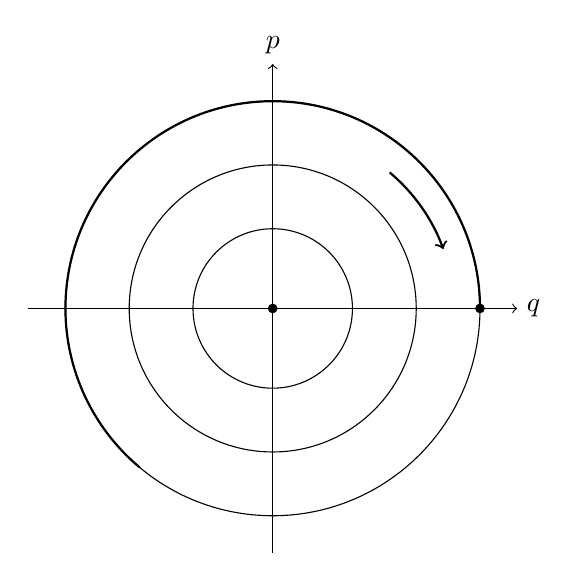
\begin{tikzpicture}[scale=1.35]
\draw[->] (-2.3,0) -- (2.3,0) node[right] {$q$};
\draw[->] (0,-2.3) -- (0,2.3) node[above] {$p$};
\draw (0,0) circle (0.75);
\draw (0,0) circle (1.35);
\draw (0,0) circle (1.95);
\draw[thick] (1.95,0) arc[start angle=0,end angle=230,radius=1.95];
\draw[->,thick] (1.10,1.28) arc[start angle=50,end angle=20,radius=1.7];
\fill (0,0) circle (1.3pt);
\fill (1.95,0) circle (1.3pt);
\end{tikzpicture}
\caption{A cleaned oscillator phase portrait. The safe content is uniform circular motion at angular speed \(\omega\); the lecture itself wavers over whether to draw the orbit clockwise or counterclockwise.}
\end{figure}

This is where the geometric interpretation becomes vivid. Every point in phase space rotates with the same angular speed \(\omega\). One may think of the whole picture as a rigid pinwheel. Or, as Susskind suggests, one may think of it as a fictitious fluid filling the plane. The fluid rotates without squeezing together and without flying apart. That is the phase-space way of seeing the absence of convergence and divergence.

At this point the lecture also answers a broader question about phase space. Is it a better representation than configuration space? Not absolutely. It serves different purposes. In phase space one sees cycles, conserved quantities, and the geometric character of the flow with unusual clarity. That is part of the power of the Hamiltonian description.

\section{Summary and Outlook}

The lecture begins with the power of the Lagrangian formalism in its most practical form. The sliding wedge shows the basic procedure: choose coordinates, write \(T-V\), compute canonical momenta, and read off the conserved quantity associated with a symmetry. The double pendulum then sharpens the lesson. Coordinate choice is partly an art, because the right coordinates make symmetry visible. In the no-gravity problem that means choosing \(\alpha\) relative to the first rod, so that \(\theta\) becomes cyclic and the conserved quantity is immediately apparent.

From there the lecture broadens into Hamiltonian mechanics. The Hamiltonian is not only the conserved energy; it is a new formulation of dynamics in terms of \(q_i\) and \(p_i\). In the harmonic oscillator, after a deliberate rescaling of variables, it becomes
\begin{equation}
H=\frac{\omega}{2}(p^2+q^2),
\end{equation}
and that makes the phase-space motion almost embarrassingly transparent: the orbits are circles, and the whole flow is a rigid rotation.

The last widening of perspective is also characteristic. The real importance of the Hamiltonian is not merely that it gives beautiful classical equations. It is that the Hamiltonian becomes central in quantum mechanics. That is why the course is going this way. And in the same spirit the lecture ends by putting potential energy ahead of force. For conservative systems it is better to think of force as derived:
\begin{equation}
\dot p_i=\frac{\partial L}{\partial q_i}=-\frac{\partial V}{\partial q_i},
\end{equation}
when \(L=T-V\) and the kinetic term carries no explicit coordinate dependence. Potential energy is the primary object; force is its derivative. That is exactly the kind of shift in viewpoint these notes have been building toward.
